\chapter{Listarakenteet}

Lista on tietorakenne, joka sisältää joukon alkioita tietyssä järjestyksessä.
Esimerkiksi $[3,7,2,5]$ on lista, jossa on neljä alkiota.
Tavallisia listan operaatioita ovat seuraavat:

\begin{itemize}
\item etsi alkio listalta
\item lisää alkio listalle
\item poista alkio listalta
\end{itemize}

Tässä luvussa tutustumme kahteen tapaan listan toteuttamiseen.
Toteutamme listan ensin taulukon avulla ja sen jälkeen
linkitettynä rakenteena.
Kuten tulemme huomaamaan, molemmissa tavoissa on omat
hyvät ja huonot puolensa.

\section{Taulukkolista}

Taulukko on tehokas tietorakenne, joka sopii hyvin listan alustaksi.
Ainoa ongelma on, että meidän täytyy päättää taulukon koko
samalla kun luomme sen emmekä voi muuttaa kokoa myöhemmin.
Esimerkiksi seuraava koodi luo taulukon, jossa on pysyvästi 10 alkiota:

\begin{code}
int[] taulu = new int[10];
\end{code}

Kuinka voimme luoda muuttuvan kokoisen listan taulukon avulla?
Ratkaisuna on varata taulukkoon \emph{ylimääräistä}
tilaa tuleville listan alkioille.
Tällä tavalla voimme luoda listan, joka pystyy laajentumaan.
Seuraavaksi käymme läpi kaksi toteutusta,
joista ensimmäisessä voimme lisätä ja poistaa alkioita
listan lopussa ja toisessa sekä listan alussa että lopussa.

\subsection{Lisäykset/poistot lopussa}

Säilytämme listaa taulukossa niin,
että tietty määrä taulukon ensimmäisiä alkioita on listan käytössä
ja loput alkiot on varattu tuleville alkioille.
Kuva \ref{fig:listau} näyttää esimerkin listan $[3,7,2,5]$ tallentamisesta taulukkoon.
Taulukossa on paikkoja kahdeksalle alkiolle, ja niistä neljä on tällä hetkellä käytössä.
Kun listan loppuun lisätään uusi alkio 6, se mahtuu taulukkoon.
Tällä tavalla alkion lisääminen listaan vie vain $O(1)$ aikaa.

\begin{figure}
\center
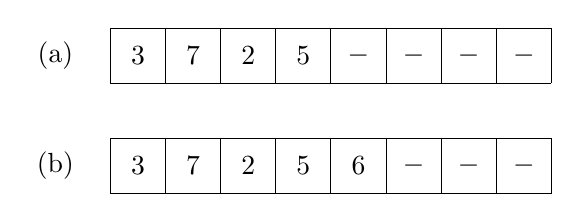
\begin{tikzpicture}[scale=0.7]
\begin{scope}
\draw (0,0) grid (8,1);
\node at (-1,0.5) {(a)};
\node at (0.5,0.5) {$3$};
\node at (1.5,0.5) {$7$};
\node at (2.5,0.5) {$2$};
\node at (3.5,0.5) {$5$};
\node at (4.5,0.5) {$-$};
\node at (5.5,0.5) {$-$};
\node at (6.5,0.5) {$-$};
\node at (7.5,0.5) {$-$};
\end{scope}
\begin{scope}[yshift=-2cm]
\draw (0,0) grid (8,1);
\node at (-1,0.5) {(b)};
\node at (0.5,0.5) {$3$};
\node at (1.5,0.5) {$7$};
\node at (2.5,0.5) {$2$};
\node at (3.5,0.5) {$5$};
\node at (4.5,0.5) {$6$};
\node at (5.5,0.5) {$-$};
\node at (6.5,0.5) {$-$};
\node at (7.5,0.5) {$-$};
\end{scope}
\end{tikzpicture}
\caption{(a) Lista $[3,7,2,5]$ tallennettuna taulukkoon. (b) Listan loppuun lisätään alkio 6.}
\label{fig:listau}
\end{figure}

Tässä on kuitenkin yksi ongelma: jossain vaiheessa koko taulukko
voi täyttyä eikä uusi listalle lisättävä alkio mahdu enää taulukkoon.
Esimerkiksi kuvassa \ref{fig:lisuus} uusi alkio 4 ei mahdu taulukkoon.
Tällöin meidän täytyy varata uusi suurempi taulukko ja
kopioida kaikki vanhan taulukon alkiot siihen.
Joudumme siis tekemään jotain seuraavanlaista,
jossa $n$ on taulukon nykyinen koko ja $m$ on varattavien
lisäpaikkojen määrä.

\begin{code}
int[] uusi = new int[n+m];
for (int i = 0; i < n; i++) {
    uusi[i] = lista[i];
}
lista = uusi;
\end{code}

Tämä on hidas operaatio, johon kuluu aikaa $O(n)$.
Olemme saaneet siis aikaan listan, jossa lisääminen vie
\emph{yleensä} aikaa $O(1)$ mutta välillä $O(n)$
uuden taulukon varaamisen ja alkioiden kopioinnin takia.

\begin{figure}
\center
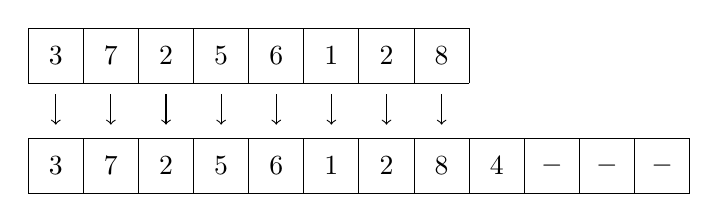
\begin{tikzpicture}[scale=0.7]
\begin{scope}
\draw (0,0) grid (8,1);
\node at (0.5,0.5) {$3$};
\node at (1.5,0.5) {$7$};
\node at (2.5,0.5) {$2$};
\node at (3.5,0.5) {$5$};
\node at (4.5,0.5) {$6$};
\node at (5.5,0.5) {$1$};
\node at (6.5,0.5) {$2$};
\node at (7.5,0.5) {$8$};
\foreach \x in {0,...,7} \draw[->] (\x+0.5,-0.2) -- (\x+0.5,-0.75);
\end{scope}
\begin{scope}[yshift=-2cm]
\draw (0,0) grid (12,1);
\node at (0.5,0.5) {$3$};
\node at (1.5,0.5) {$7$};
\node at (2.5,0.5) {$2$};
\node at (3.5,0.5) {$5$};
\node at (4.5,0.5) {$6$};
\node at (5.5,0.5) {$1$};
\node at (6.5,0.5) {$2$};
\node at (7.5,0.5) {$8$};
\node at (8.5,0.5) {$4$};
\node at (9.5,0.5) {$-$};
\node at (10.5,0.5) {$-$};
\node at (11.5,0.5) {$-$};
\end{scope}
\end{tikzpicture}
\caption{Taulukkoon ei mahdu enää uutta alkiota. Meidän täytyy varata uusi suurempi taulukko
ja kopioida vanhan taulukon sisältö sinne.}
\label{fig:lisuus}
\end{figure}

Jotta rakenne olisi käyttökelpoinen, meidän täytyy varmistaa,
että hidas $O(n)$-operaatio ei esiinny liian usein.
Tämä on mahdollista, kun varaamme uuden taulukon aina reilusti aiempaa suuremmaksi.
Tarkemmin ottaen yksi mahdollinen tapa on varata aina uusi taulukko niin,
että sen koko on \emph{kaksinkertainen} vanhaan taulukkoon nähden.
Kun toimimme näin, jokaisen alkion lisääminen listalle vie
\emph{keskimäärin} vain $O(1)$ aikaa.

Voimme ajatella asian näin: jokainen listalle lisättävä alkio
maksaa pääsy\-maksuna kolme euroa.
Tästä yksi euro menee listalle liittymiseen ja kaksi euroa jäävät säästöön.
Sitten kun aikanaan listalle täytyy varata suurempi taulukko,
jokainen viime erässä lisätty alkio maksaa yhden euron omasta siirrostaan
ja yhden euron aiemmin lisätyn alkion siirrosta.
Koska taulukon koko kaksinkertaistuu joka vaiheessa,
kolmen euron kiinteä pääsymaksu riittää siihen, että kaikki tulevat
siirrot saadaan kustannettua.

\begin{figure}
\center
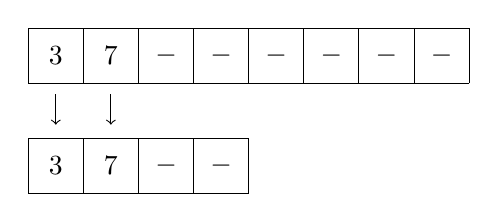
\begin{tikzpicture}[scale=0.7]
\begin{scope}
\draw (0,0) grid (8,1);
\node at (0.5,0.5) {$3$};
\node at (1.5,0.5) {$7$};
\node at (2.5,0.5) {$-$};
\node at (3.5,0.5) {$-$};
\node at (4.5,0.5) {$-$};
\node at (5.5,0.5) {$-$};
\node at (6.5,0.5) {$-$};
\node at (7.5,0.5) {$-$};
\foreach \x in {0,...,1} \draw[->] (\x+0.5,-0.2) -- (\x+0.5,-0.75);
\end{scope}
\begin{scope}[yshift=-2cm]
\draw (0,0) grid (4,1);
\node at (0.5,0.5) {$3$};
\node at (1.5,0.5) {$7$};
\node at (2.5,0.5) {$-$};
\node at (3.5,0.5) {$-$};
\end{scope}
\end{tikzpicture}
\caption{Poistojen jälkeen taulukon koko on käynyt tarpeettoman suureksi,
ja puolitamme taulukon koon.}                                                                        
\label{fig:lispoi}
\end{figure}

Voimme poistaa alkion listan lopusta aina $O(1)$-ajassa,
koska taulukon kokoa ei tarvitse koskaan suurentaa.
Tässä voi kuitenkin tulla ongelmaksi, että monien poistojen
jälkeen taulukossa on turhan paljon tyhjää tilaa lopussa.
Voimme soveltaa tässä käänteisesti samaa ideaa kuin lisäämisessä:
jos poistamisen jälkeen vain \emph{neljännes} taulukosta on käytössä,
puolitamme taulukon koon.
Kuva \ref{fig:lispoi} näyttää esimerkin tällaisesta tilanteesta.
Tällä tavalla poistamiset vievät keskimäärin aikaa $O(1)$.

Miksi sitten emme voisi varata heti aluksi niin suurta taulukkoa,
että lopullinen lista mahtuisi siihen varmasti?
Tässä olisi huonona puolena, että listamme tuhlaisi paljon muistia.
Ohjelmassa saattaa olla samaan aikaan käytössä monia listoja,
ja haluamme, että listan varaama taulukko on samaa kokoluokkaa
kuin listan todellinen sisältö.

\subsection{Lisäykset/poistot alussa ja lopussa}

Seuraava tavoitteemme on luoda lista,
joka sallii alkioiden lisäämisen ja poistamisen
sekä listan alussa että lopussa.
Voimme menetellä lähes samalla tavalla kuin ennenkin,
kunhan luovumme yhdestä periaatteesta:
taulukon ensimmäinen alkio ei enää välttämättä
ole listan ensimmäinen alkio.
Sen sijaan listan ensimmäisen ja
viimeisen alkion kohdat taulukossa vaihtelevat ja listan sisältö
voi jatkua taulukon lopusta taulukon alkuun.

\begin{figure}
\center
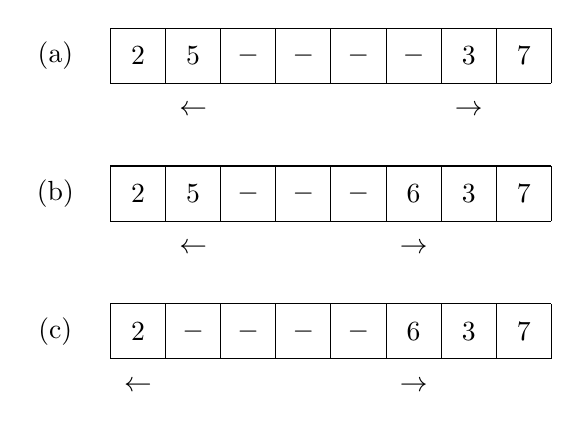
\begin{tikzpicture}[scale=0.7]
\begin{scope}
\draw (0,0) grid (8,1);
\node at (-1,0.5) {(a)};
\node at (0.5,0.5) {$2$};
\node at (1.5,0.5) {$5$};
\node at (2.5,0.5) {$-$};
\node at (3.5,0.5) {$-$};
\node at (4.5,0.5) {$-$};
\node at (5.5,0.5) {$-$};
\node at (6.5,0.5) {$3$};
\node at (7.5,0.5) {$7$};
\node at (1.5,-0.5) {$\leftarrow$};
\node at (6.5,-0.5) {$\rightarrow$};
\end{scope}
\begin{scope}[yshift=-2.5cm]
\draw (0,0) grid (8,1);
\node at (-1,0.5) {(b)};
\node at (0.5,0.5) {$2$};
\node at (1.5,0.5) {$5$};
\node at (2.5,0.5) {$-$};
\node at (3.5,0.5) {$-$};
\node at (4.5,0.5) {$-$};
\node at (5.5,0.5) {$6$};
\node at (6.5,0.5) {$3$};
\node at (7.5,0.5) {$7$};
\node at (1.5,-0.5) {$\leftarrow$};
\node at (5.5,-0.5) {$\rightarrow$};
\end{scope}
\begin{scope}[yshift=-5cm]
\draw (0,0) grid (8,1);
\node at (-1,0.5) {(c)};
\node at (0.5,0.5) {$2$};
\node at (1.5,0.5) {$-$};
\node at (2.5,0.5) {$-$};
\node at (3.5,0.5) {$-$};
\node at (4.5,0.5) {$-$};
\node at (5.5,0.5) {$6$};
\node at (6.5,0.5) {$3$};
\node at (7.5,0.5) {$7$};
\node at (0.5,-0.5) {$\leftarrow$};
\node at (5.5,-0.5) {$\rightarrow$};
\end{scope}
\end{tikzpicture}
\caption{(a) Lista $[3,7,2,5]$ tallennettuna taulukkoon.
(b) Listan alkuun lisätään alkio 6.
(c) Listan lopusta poistetaan alkio 5.}
\label{fig:lismol}
\end{figure}

Kuva \ref{fig:lismol} näyttää esimerkin listan $[3,7,2,5]$
uudesta tallennustavasta.
Merkki $\rightarrow$ osoittaa kohdan, josta lista alkaa,
ja merkki $\leftarrow$ osoittaa kohdan, johon lista päättyy.
Kun haluamme lisätä alkion listan alkuun,
siirrymme vasemmalle kohdasta $\rightarrow$,
ja kun haluamme lisätä alkion listan loppuun,
siirrymme oikealle kohdasta $\leftarrow$.
Kun haluamme poistaa alkioita listasta,
menettelemme käänteisesti.

\begin{figure}
\center
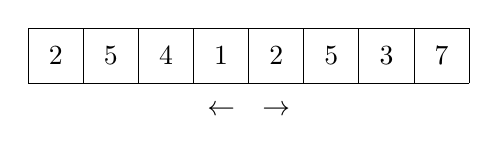
\begin{tikzpicture}[scale=0.7]
\begin{scope}
\draw (0,0) grid (8,1);
\node at (0.5,0.5) {$2$};
\node at (1.5,0.5) {$5$};
\node at (2.5,0.5) {$4$};
\node at (3.5,0.5) {$1$};
\node at (4.5,0.5) {$2$};
\node at (5.5,0.5) {$5$};
\node at (6.5,0.5) {$3$};
\node at (7.5,0.5) {$7$};
\node at (3.5,-0.5) {$\leftarrow$};
\node at (4.5,-0.5) {$\rightarrow$};
\end{scope}
\end{tikzpicture}
\caption{Lista $[2,5,3,7,2,5,4,1]$ täyttää koko taulukon, emmekä voi lisätä uutta alkiota.
Ratkaisuna on varata suurempi taulukko.}
\label{fig:lismol2}
\end{figure}

Jos kohdat $\rightarrow$ ja $\leftarrow$ ovat vierekkäin,
taulukko on täynnä, emmekä voi enää lisätä uutta alkiota
listan alkuun tai loppuun.
Kuva \ref{fig:lismol2} näyttää esimerkin tällaisesta tilanteesta.
Tällöin meidän täytyy varata uusi suurempi taulukko,
johon listan sisältö siirretään.
Voimme menetellä samalla tavalla kuin aiemmin ja
kaksinkertaistaa taulukon koon joka vaiheessa,
jolloin operaatiot vievät keskimäärin aikaa $O(1)$.

\section{Linkitetty lista}

Linkitetty lista muodostuu solmuista, joista jokainen sisältää
yhden listan alkion.
Yhteen suuntaan linkitetyssä listassa jokaisessa
solmussa on viittaus listan seuraavaan solmuun.
Kahteen suuntaan linkitetyssä listassa taas
solmut viittaavat sekä listan seuraavaan että edelliseen solmuun.
Viittausten avulla pystymme liikkumaan listassa.

\begin{figure}
\center
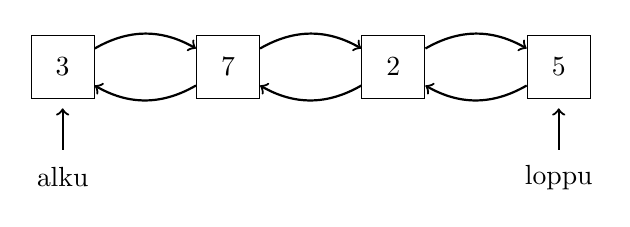
\begin{tikzpicture}[scale=0.7]
\begin{scope}
\node[draw, rectangle, minimum size=8mm] (1) at (0,0) {$3$};
\node[draw, rectangle, minimum size=8mm] (2) at (3,0) {$7$};
\node[draw, rectangle, minimum size=8mm] (3) at (6,0) {$2$};
\node[draw, rectangle, minimum size=8mm] (4) at (9,0) {$5$};
\path[draw,thick,->] (1) edge [bend left] (2);
\path[draw,thick,->] (2) edge [bend left] (3);
\path[draw,thick,->] (3) edge [bend left] (4);
\path[draw,thick,->] (4) edge [bend left] (3);
\path[draw,thick,->] (3) edge [bend left] (2);
\path[draw,thick,->] (2) edge [bend left] (1);
\node at (0,-2) {alku};
\node at (9,-2) {loppu};
\path[draw,thick,->] (0,-1.5) -- (0,-0.75);
\path[draw,thick,->] (9,-1.5) -- (9,-0.75);
\end{scope}
\end{tikzpicture}
\caption{Kahteen suuntaan linkitetty lista, joka sisältää alkiot $[3,7,2,5]$.}
\label{fig:linlis}
\end{figure}

Kuvassa \ref{fig:linlis} on esimerkkinä kahteen suuntaan linkitetty lista,
joka sisältää alkiot $[3,7,2,5]$.
Jokainen alkio viittaa seuraavaan ja edelliseen alkioon,
minkä ansiosta pystymme liikkumaan listassa.
Lisäksi tiedossamme on viittaukset listan alkuun ja loppuun.
Voimme esimerkiksi käydä listan läpi aloittamalla alusta
ja siirtymällä aina seuraavaan solmuun askel kerrallaan.

\subsection{Linkitetyn rakenteen toteuttaminen}

Jokaisessa ohjelmointikielessä on omat keinonsa
linkitetyn rakenteen toteuttamiseen.
Javassa voimme toteuttaa linkitetyn rakenteen niin,
että jokainen solmu on oma olionsa.
Esimerkiksi voimme toteuttaa seuraavan luokan \texttt{Node},
jonka oliot toimivat linkitetyn listan solmuina:

\begin{code}
public class Solmu {
    public int arvo;
    public Solmu seuraava;
    public Solmu edellinen;

    public Solmu(int arvo, Solmu seuraava, Solmu edellinen) {
        this.arvo = arvo;
        this.seuraava = seuraava;
        this.edellinen = edellinen;
    }
}
\end{code}

Tässä kenttä \texttt{arvo} kertoo solmun arvon,
kenttä \texttt{seuraava} osoittaa seuraavaan solmuun
ja kenttä \texttt{edellinen} osoittaa edelliseen solmuun.
Jos seuraavaa tai edellistä solmua ei ole,
viittauksen tilalla on arvo \texttt{null}.
Tämän luokan avulla voisimme luoda linkitetyn listan $[3,7,2,5]$
seuraavasti:

\begin{code}
Solmu s1, s2, s3, s4;
s1 = new Solmu(3, s2, null);
s2 = new Solmu(7, s3, s1);
s3 = new Solmu(2, s4, s2);
s4 = new Solmu(5, null, s3);
\end{code}

Tämän jälkeen voisimme käydä listan läpi näin alusta loppuun:

\begin{code}
Solmu s = s1;
while (s != null) {
    System.out.println(s.arvo);
    s = s.seuraava;
}
\end{code}

Koodin tulostus on seuraava:

\begin{code}
3
7
2
5
\end{code}

\subsection{Listan operaatiot}

Linkitetyn listan etuna on,
että voimme lisätä ja poistaa
alkioita $O(1)$-ajassa kaikissa listan kohdissa.
Kun haluamme lisätä listalle alkion,
luomme ensin uuden solmun ja muutamme sitten
sen vieressä olevien solmujen viittauksia niin,
että ne viittaavat uuteen solmuun.
Vastaavasti kun haluamme poistaa alkion,
muutamme viittauksia niin, että solmu ohitetaan.

\begin{figure}
\center
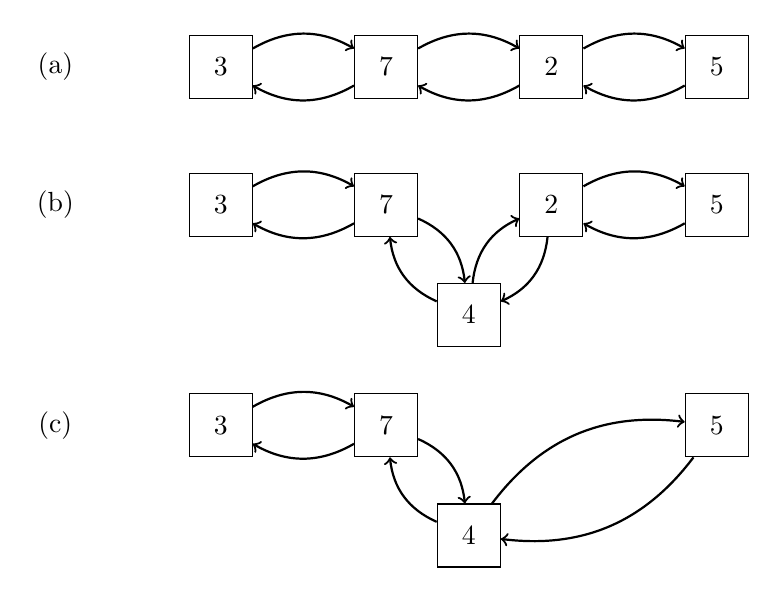
\begin{tikzpicture}[scale=0.7]
\begin{scope}
\node at (-3,0) {(a)};
\node[draw, rectangle, minimum size=8mm] (1) at (0,0) {$3$};
\node[draw, rectangle, minimum size=8mm] (2) at (3,0) {$7$};
\node[draw, rectangle, minimum size=8mm] (3) at (6,0) {$2$};
\node[draw, rectangle, minimum size=8mm] (4) at (9,0) {$5$};
\path[draw,thick,->] (1) edge [bend left] (2);
\path[draw,thick,->] (2) edge [bend left] (3);
\path[draw,thick,->] (3) edge [bend left] (4);
\path[draw,thick,->] (4) edge [bend left] (3);
\path[draw,thick,->] (3) edge [bend left] (2);
\path[draw,thick,->] (2) edge [bend left] (1);
\end{scope}
\begin{scope}[yshift=-2.5cm]
\node at (-3,0) {(b)};
\node[draw, rectangle, minimum size=8mm] (1) at (0,0) {$3$};
\node[draw, rectangle, minimum size=8mm] (2) at (3,0) {$7$};
\node[draw, rectangle, minimum size=8mm] (3) at (6,0) {$2$};
\node[draw, rectangle, minimum size=8mm] (4) at (9,0) {$5$};
\node[draw, rectangle, minimum size=8mm] (5) at (4.5,-2) {$4$};
\path[draw,thick,->] (1) edge [bend left] (2);
\path[draw,thick,->] (2) edge [bend left] (5);
\path[draw,thick,->] (5) edge [bend left] (3);
\path[draw,thick,->] (3) edge [bend left] (4);
\path[draw,thick,->] (4) edge [bend left] (3);
\path[draw,thick,->] (3) edge [bend left] (5);
\path[draw,thick,->] (5) edge [bend left] (2);
\path[draw,thick,->] (2) edge [bend left] (1);
\end{scope}
\begin{scope}[yshift=-6.5cm]
\node at (-3,0) {(c)};
\node[draw, rectangle, minimum size=8mm] (1) at (0,0) {$3$};
\node[draw, rectangle, minimum size=8mm] (2) at (3,0) {$7$};
\node[draw, rectangle, minimum size=8mm] (4) at (9,0) {$5$};
\node[draw, rectangle, minimum size=8mm] (5) at (4.5,-2) {$4$};
\path[draw,thick,->] (1) edge [bend left] (2);
\path[draw,thick,->] (2) edge [bend left] (5);
\path[draw,thick,->] (5) edge [bend left] (4);
\path[draw,thick,->] (4) edge [bend left] (5);
\path[draw,thick,->] (5) edge [bend left] (2);
\path[draw,thick,->] (2) edge [bend left] (1);
\end{scope}
\end{tikzpicture}
\caption{(a) Alkuperäinen lista $[3,7,2,5]$.
(b) Listan keskelle lisätään alkio $4$.
(c) Listasta poistetaan alkio $2$.}
\label{fig:lismuu}
\end{figure}

Kuva \ref{fig:lismuu} näyttää esimerkin linkitetyn listan käsittelystä.
Listan sisältönä on aluksi $[3,7,2,5]$.
Sitten lisämme listan keskelle alkion 4,
jolloin luomme ensin uuden solmun alkiolle ja muutamme
sitten viittauksia alkioiden 7 ja 2 välillä niin,
että alkio 4 tulee niiden väliin.
Lopuksi poistamme listasta alkion 2, jolloin yhdistämme
alkiot 4 ja 5 suoraan toisiinsa.

Koska meillä on muistissa viittaukset listan alkuun ja loppuun,
pääsemme niihin tehokkaasti.
Sen sijaan jos haluamme päästä johonkin muuhun listan kohtaan,
meidän tulee aloittaa alusta tai lopusta ja kulkea askel
kerrallaan viittauksia seuraten.
Niinpä tiettyyn listan kohtaan pääseminen vie aikaa $O(n)$.
Joudumme tekemään näin, koska listan alkiot voivat olla
tallessa eri puolilla muistia eikä meillä ole suoraa keinoa
päästä niihin.

\section{Javan toteutukset}

Javan standardikirjastossa on monia listojen toteutuksia,
jotka pohjautuvat taulukkolistaan tai linkitettyyn listaan.
Seuraavaksi tutustumme käytännössä hyödyllisimpiin
Javan toteutuksista.

\subsection{\texttt{ArrayList}-rakenne}

\texttt{ArrayList}-rakenne toteuttaa taulukkolistan,
joka sallii tehokkaat lisäykset ja poistot listan lopussa.
Esimerkkinä seuraava koodi luo listan, lisää siihen alkiot
1, 2 ja 3 ja tulostaa listan sisällön.
Sitten koodi poistaa listan viimeisen alkion ja
tulostaa uudestaan listan sisällön.

\begin{code}
ArrayList<Integer> lista = new ArrayList<>();
lista.add(1);
lista.add(2);
lista.add(3);
System.out.println(lista); // [1, 2, 3]
lista.remove(2);
System.out.println(lista); // [1, 2]
\end{code}

Metodit \texttt{add} ja \texttt{remove}
toimivat keskimäärin ajassa $O(1)$,
kun käytämme niitä listan lopussa.
Huomaa, että metodille \texttt{remove} täytyy ilmoittaa,
mistä kohdasta poistamme alkion.
Lisäksi voimme käyttää listaa tehokkaasti taulukon tavoin
ja käsitellä tietyssä kohdassa olevaa alkiota
metodeilla \texttt{get} ja \texttt{set}.
Esimerkiksi seuraava koodi tulostaa ensin
listan kohdassa 1 olevan alkion ja muuttaa sitten
sen arvoksi 5.

\begin{code}
System.out.println(lista.get(1)); // 2
lista.set(1,5);
System.out.println(lista); // [1, 5, 3]
\end{code}

Luokassa \texttt{Collections} on hyödyllisiä metodeita
listan käsittelyyn.
Seuraava koodi järjestää ensin listan,
muuttaa sitten sen järjestyksen käänteiseksi
ja sekoittaa lopuksi järjestyksen.

\begin{code}
Collections.sort(lista);
Collections.reverse(lista);
Collections.shuffle(lista);
\end{code}

\subsection{\texttt{ArrayDeque}-rakenne}

\texttt{ArrayDeque}-rakenne toteuttaa taulukkolistan,
joka sallii tehokkaat lisäykset ja poistot
sekä listan alussa että lopussa.
Seuraava koodi esittelee rakenteen käyttämistä:

\begin{code}
ArrayDeque<Integer> lista = new ArrayDeque<>();
lista.addLast(1);
lista.addFirst(2);
lista.addLast(3);
System.out.println(lista); // [2, 1, 3]
lista.removeFirst();
System.out.println(lista); // [1, 3]
\end{code}

Rakenteen rajoituksena on, että voimme käsitellä
vain listan ensimmäistä ja viimeistä alkiota mutta
emme listan muita alkioita.
Voimme käyttää metodeita \texttt{getFirst} ja \texttt{getLast}
hakemaan listan ensimmäisen ja viimeisen alkion,
mutta rakenteessa ei ole yleistä metodia \texttt{get},
jolla voisimme hakea minkä tahansa alkion listalta.

\subsection{\texttt{LinkedList}-rakenne}

\texttt{LinkedList}-rakenne toteuttaa kaksisuuntaisen
linkitetyn listan, jossa voimme helposti lisätä ja poistaa
alkioita listan alussa ja lopussa.
Seuraava koodi esittelee asiaa:

\begin{code}
LinkedList<Integer> lista = new LinkedList<>();
lista.addLast(1);
lista.addFirst(2);
lista.addLast(3);
System.out.println(lista); // [2,1,3]
lista.removeFirst();
System.out.println(lista); // [1,3]
\end{code}

Jos haluamme tehdä lisäyksiä ja poistoja muualla listassa,
meillä täytyy olla \emph{iteraattori}, joka osoittaa haluttuun kohtaan.
Seuraava koodi luo iteraattorin, joka osoittaa ensin listan alkuun.
Sitten se siirtää iteraattoria kaksi askelta eteenpäin ja
lisää alkion 5 iteraattorin kohdalle eli listan
toisen ja kolmannen alkion väliin.

\begin{code}
ListIterator<Integer> x = lista.listIterator(0);
x.next();
x.next();
x.add(5);
\end{code}

\texttt{LinkedList} tarjoaa myös metodeita,
joiden avulla voi käsitellä tietyssä kohdassa listaa olevaa alkiota
(esimerkiksi metodit \texttt{get} ja \texttt{set}).
Nämä metodit vievät kuitenkin aikaa $O(n)$,
koska joudumme kulkemaan ensin oikeaan kohtaan listan
alusta tai lopusta.
Tämän vuoksi \texttt{LinkedList} ei ole hyvä valinta,
jos haluamme käsitellä alkioita kohdan perusteella.

\section{Tehokkuusvertailu}

Seuraavaksi teemme kaksi testiä, joiden tarkoituksena on
antaa kuvaa, kuinka tehokkaita rakenteita
taulukkolista ja linkitetty lista ovat käytännössä.
Ensimmäisessä testissä keskitymme listan läpikäyntiin ja otamme
vertailun mukaan myös tavallisen taulukon.
Toisessa testissä mittaamme nopeutta, kun muokkaamme listaa
sen alussa ja lopussa.

\subsection{Testi 1: Läpikäynti}

Käytämme testiaineistona listaa, jossa on $n$ satunnaista
kokonaislukua väliltä $1 \dots 100$.
Laskemme jokaiselle kokonaisluvulle $1 \dots 100$,
montako kertaa se esiintyy listalla.

Koska listan koko on kiinteä, voimme toteuttaa vertailukohtana
ratkaisun, joka käyttää tavallista taulukkoa.
Seuraava metodi selvittää, kuinka monta kertaa luku $x$
esiintyy taulukossa.

\begin{code}
int kerrat(int[] taulu, int x) {
    int tulos = 0;
    for (int i = 0; i < n; i++) {
        if (taulu[i] == x) tulos++;
    }
    return tulos;
}
\end{code}

\texttt{ArrayList}- ja \texttt{LinkedList}-rakenteen
testaamiseksi käytämme seuraavaa metodia.
Sama metodi toimii molemmille rakenteille,
koska listan tyypiksi on annettu \texttt{List}.

\begin{code}
int kerrat(List<Integer> lista, int x) {
    int tulos = 0;
    for (Integer luku : lista) {
        if (luku == x) tulos++;
    }
    return s;
}
\end{code}

\begin{table}
\center
\begin{tabular}{rrrr}
taulukon koko $n$ & taulukko & \texttt{ArrayList} & \texttt{LinkedList} \\
\hline
$10^6$ & 0.06 s & 0.15 s & 0.44 s \\
$2 \cdot 10^6$ & 0.13 s & 0.30 s & 0.90 s \\
$4 \cdot 10^6$ & 0.26 s & 0.60 s & 1.66 s \\
$8 \cdot 10^6$ & 0.53 s & 1.30 s & 3.40 s \\
$16 \cdot 10^6$ & 1.33 s & 3.39 s & 7.99 s \\
\end{tabular}
\caption{Algoritmien suoritusaikojen vertailu.}
\label{tab:kerver}
\end{table}

Taulukko \ref{tab:kerver} näyttää testin tulokset.
Osoittautuu, että tässä testissä taulukko toimii noin
2,5 kertaa nopeammin kuin \texttt{ArrayList}.
Tämä on kiinnostava havainto, koska \texttt{ArrayList}
perustuu taulukkoon eikä sen koko muutu testin aikana.
Toisaalta \texttt{ArrayList} toimii puolestaan noin
2,5 kertaa nopeammin kuin \texttt{LinkedList}.

\subsection{Testi 2: Lisäykset ja poistot}

Toisessa testissä vertaamme \texttt{ArrayDeque}- ja \texttt{LinkedList}-rakenteita.
Käymme läpi luvut $1,2,\dots,n$.
Luvun ollessa jaollinen kolmella poistamme sen listan alusta
ja muuten lisäämme sen listan loppuun.
Lopuksi laskemme listan lukujen summan.

Seuraava koodi toteuttaa testin parametrina annetulle tyhjälle listalle.
Sekä \texttt{ArrayDeque} että \texttt{LinkedList} toteuttavat
rajapinnan \texttt{Deque}, joten voimme käyttää samaa koodia
kummankin rakenteen testaamiseen.

\begin{code}
long summa(Deque<Integer> lista) {
    for (int i = 1; i <= n; i++) {
        if (i%3 == 0) lista.removeFirst();
        else lista.addLast(i);
    }
    long summa = 0;
    for (Integer x : lista) summa += x;
    return summa;
}
\end{code}

Taulukko \ref{tab:lispoi} näyttää testin tulokset.
Osoittautuu, että \texttt{ArrayDeque}-raken\-ne on
2–3 kertaa nopeampi kuin \texttt{LinkedList}-rakenne.

\begin{table}
\center
\begin{tabular}{rrr}
parametri $n$ & \texttt{ArrayDeque} & \texttt{LinkedList} \\
\hline
$10^6$ & 0.01 s & 0.02 s \\
$2 \cdot 10^6$ & 0.02 s & 0.08 s \\
$4 \cdot 10^6$ & 0.08 s & 0.14 s \\
$8 \cdot 10^6$ & 0.27 s & 0.44 s \\
$16 \cdot 10^6$ & 0.88 s & 3.13 s \\
\end{tabular}
\caption{Algoritmien suoritusaikojen vertailu.}
\label{tab:lispoi}
\end{table}

\subsection{Linkitetyn listan käyttö}

Jokaisessa tietorakenteessa on omat hyvät ja huonot puolensa,
ja kaikille on tietyt käyttötarkoituksensa.
Linkitetty lista muodostaa kuitenkin poikkeuksen tähän sääntöön:
on äärimmäisen harvoja tilanteita, jolloin sitä kannattaisi
käyttää taulukkolistan sijasta.

\begin{figure}
\center
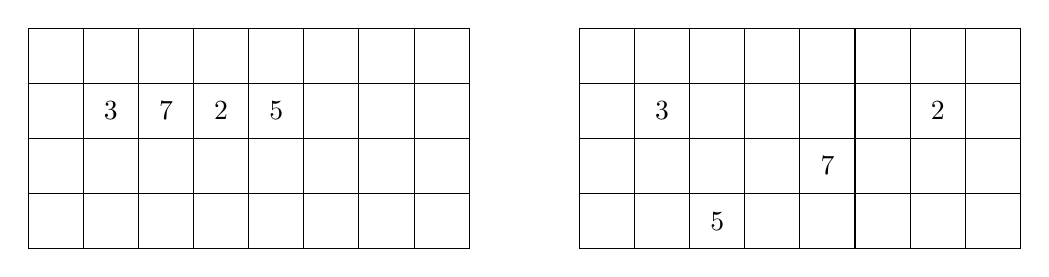
\begin{tikzpicture}[scale=0.7]
\begin{scope}
\draw (0,0) grid (8,4);
\node at (1.5,2.5) {3};
\node at (2.5,2.5) {7};
\node at (3.5,2.5) {2};
\node at (4.5,2.5) {5};
\end{scope}
\begin{scope}[xshift=10cm]
\draw (0,0) grid (8,4);
\node at (1.5,2.5) {3};
\node at (4.5,1.5) {7};
\node at (6.5,2.5) {2};
\node at (2.5,0.5) {5};
\end{scope}
\end{tikzpicture}
\caption{Taulukkolista ja linkitetty lista tietokoneen muistissa.}
\label{fig:taulin}
\end{figure}

Syynä tähän on, että nykyaikaiset tietokoneet
\emph{suosivat} taulukkolistan käyttämistä linkitetyn listan sijaan.
Kuvassa \ref{fig:taulin} näkyy, miten taulukkolista ja linkitetty lista
asettuvat tietokoneen muistissa.
Taulukkolistan alkiot ovat peräkkäin, kun taas linkitetyn
listan alkiot voivat olla eri puolilla muistia sekalaisessa
järjestyksessä.
Nykyaikaisen prosessorin välimuistit ja komentojen ennustus
on toteutettu niin, että ne ovat parhaimmillaan silloin,
kun tieto on tallennettu muistissa peräkkäin -- eli juuri kuten
taulukkolistassa.
Tämä näkyy käytännössä siinä, että taulukkolistan käsittely on selvästi
nopeampaa kuin linkitetyn listan käsittely.

Linkitetyllä listalla on silti yksi ominaisuus,
joka puuttuu taulukkolistasta: voimme tehokkaasti
lisätä ja poistaa alkioita listan keskellä.
Tämä kuitenkin vaatii sen, että meillä on valmiiksi
iteraattori haluttuun kohtaan listaa,
mikä on käytännössä harvinaista.